%!TEX root = ../book.tex
\section{Differential Kinematics}\label{sec:kinematics:diff}

The two-link arm in Figure~\ref{fig:fwk2dofarm} involved only two free parameters, but was already pretty complex to solve analytically if the end-effector pose was not specified.
One can imagine that things become very hard with more degrees of freedom or more complex geometries (mechanisms in which some axes intersect are simpler to solve than others, for example).
It is worth noting that, so far, we have analyzed the geometry of motion of a robot at its simplest level of abstraction, i.e. in the space of positions. Despite its potential, this abstraction becomes quickly ineffective at modeling complex behaviors, because it does not incorporate any notion of time.
In order to include a notion of temporal evolution of the robot configuration, it is convenient to shift toward a slightly more complex abstraction, that is the space of generalized velocities. This modeling is called \textsl{differential kinematics}\index{Differential Kinematics}, as velocities are the derivative (i.e. the differential) of positions.
Similarly to before, with ``generalized velocities'' we mean ``any velocity-equivalent quantity needed to describe the element'', as we will detail below.

\subsection{Forward Differential Kinematics}\label{sec:kinematics:diff:fwd}

Forward differential kinematics deals with the problem of computing an expression that relates the generalized velocities at the joints (i.e. the ``speed'' of our motors) to the generalized velocity of the robot's end-effector. In all, it is the corresponding differential version of \cref{sec:kinematics:fwd}.
% This is known as \textsl{Differential Kinematics}\index{Differential Kinematics}, as we are operating in the space of velocities, which are the derivative of positions.
Let the translational speed of a robot be given by:
\begin{equation}
v=\left[\begin{array}{c}
\dot{x}\\
\dot{y}\\
\dot{z}
\end{array}
\right].
\end{equation}
As the robot can potentially not only translate, but also rotate, we also need to specify its angular velocity. Let these velocities be given as a vector
\begin{equation}
\omega=\left[\begin{array}{c}
\omega_x\\
\omega_y\\
\omega_z
\end{array}
\right].
\end{equation}
We can now write translational and rotational velocities in a $6\times1$ generalized velocity vector as $\nu = [v \ \omega]^T$.
This notation is also called a \textsl{velocity twist}.\index{Twist (velocity)}\index{Velocity Twist} %By convention, the speed of rotation is given by the magnitude (or length) of this vector.
Let the generalized configuration in joint space (i.e. joint angles/positions) be $q=[q_1, \ldots, q_n]^T$; therefore, we can define the set of joint speeds as $\dot{q}=[\dot{q}_1, \ldots, \dot{q}_n]^T$.
%
We now want to compute the differential kinematics version of \cref{eq:kinematics:forward}, and in this case relate joint velocities $\dot{q}$ with end-effector velocities $[v \ \omega]^T$. A simple derivation with respect to time of \cref{eq:kinematics:forward} gives:
\begin{equation}\label{eq:kinematics:diff:fwd:short}
\nu = [v \quad \omega]^T=J(q)\cdot [\dot{q}_1,\ldots,\dot{q}_n]^T = J(q) \cdot \dot{q} \ ,
\end{equation}
which is our forward kinematics equation. $J(q)$ is known as the \textsl{Jacobian matrix}\index{Jacobian Matrix}, is function of the joint configuration $q$, and contains all the partial derivatives of $f$ that relate every joint angle to every velocity. In practice, $J$ looks like the following:

\begin{equation}\label{eq:kinematics:diff:fwd}
\nu = \left[\begin{array}{c}v\\\omega\end{array}\right]=
\left[\begin{array}{c}\dot{x}\\
\dot{y}\\
\dot{z}\\
\omega_x\\
\omega_y\\
\omega_z\end{array}\right]=
\left[\begin{array}{cccc}\frac{\partial{x}}{\partial{q_1}} & \frac{\partial{x}}{\partial{q_2}} & \ldots & \frac{\partial{x}}{\partial{q_n}}\\\frac{\partial{y}}{\partial{q_1}} & \frac{\partial{y}}{\partial{q_2}} & \ldots & \frac{\partial{y}}{\partial{q_n}}\\\vdots & \vdots & \vdots & \vdots\\\frac{\partial{\omega_z}}{\partial{q_1}} & \frac{\partial{\omega_z}}{\partial{q_2}} & \ldots & \frac{\partial{\omega_z}}{\partial{q_n}}\end{array}\right]\left[\begin{array}{c}\dot{q}_1\\\vdots\\\dot{q}_n\end{array}\right] = J (q) \cdot \dot{q}
\end{equation}

This notation is important as it tells us how small changes in joint space will affect the end-effector's position in Cartesian space. Better yet, the forward kinematics of a mechanism can always be calculated, as well as their analytical derivatives, allowing us to calculate numerical values for the entries of matrix $J$ for every possible joint angle/position.

\subsection{Forward Kinematics of a Differential Wheels Robot}\label{sec:kinematics:fwk:mobile}

Whereas the pose of a robotic manipulator is uniquely defined by its joint angles---which can be made available using encoders in almost real-time, see \cref{sec:sensors:encoders}---this is not the case for a mobile robot.
Here, the encoder values simply refer to wheel orientation and need to be integrated over time in order to assess the robot's position with respect to the worlds frame of reference; as we will later see, this is a great source of uncertainty.
What complicates matters is that for so-called \textsl{non-holonomic} systems, it is not sufficient to simply measure the distance that each wheel traveled, but also when each movement was executed.

\begin{figure}[!t]
    \small
    \centering
    % 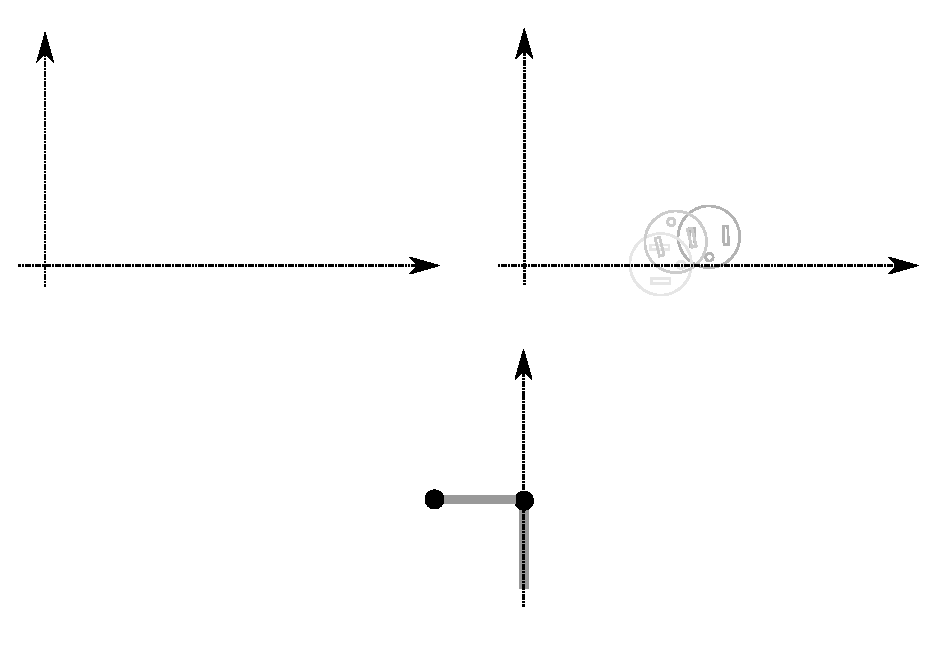
\includegraphics[width=0.95\textwidth]{figs/holonomy.png}
    \def\svgwidth{\textwidth}
    \import{./figs/kinematics/}{holonomy.pdf_tex}
    \caption{Configuration or joint space (left) and workspace or operational space (right) for a non-holonomic mobile robot (top) and a holonomic manipulator (bottom). Closed trajectories in configuration space result in closed trajectories in the workspace if the robot's kinematics is holonomic.}
    \label{fig:holonomy}
\end{figure}

A system is non-holonomic\index{Non-holonomic}\index{Holonomic} when closed trajectories in its configuration space may not have it return to its original state (reminder: the configuration or joint space space of a two-link robotic arm is spanned by the possible values of each angle).
A simple arm is holonomic because each joint position corresponds to a unique position in space:
going through whatever trajectory that comes back to the starting point in configuration space, will put the robot's end-effector at the exact same position in operational space.
A train on a track is holonomic: moving its wheels backwards by the same amount they have been moving forward brings the train to the exact same position in space.
A car and a differential-wheel robot are non-holonomic vehicles: performing a straight line and then a right-turn leads to the same amount of wheel rotation than doing a right turn first and then going in a straight line; however getting the robot to its initial position requires not only to rewind both wheels by the same amount, but also getting their relative speeds right.
The configuration and corresponding workspace trajectories for a non-holonomic and a holonomic robot are shown in \cref{fig:holonomy}.
Here, a robot first moves on a straight line, i.e. both wheels turn an equal amount.
Then, the left wheel remains fixed and only the right wheel turns forward.
Then, the right wheel remain fixed and the left wheel turns backward.
Finally, the right wheel turns backward, arriving at the initial encoder values (zero).
Yet, the robot does not return to its origin. Performing a similar trajectory in the configuration space of a two-link manipulator instead, lets the robot return to its initial position.

It should be clear by now that for a mobile robot, not only traveled distance per wheel matters, but also the \textsl{speed} of each wheel as a function of time.
Interestingly however, this information was not required to uniquely determine the pose of a manipulating arm.
Let's introduce the following conventions.
We will establish a world coordinate system $\{I\}$---which is known as the inertial frame by convention (see \cref{fig:mobilerobot}).
We establish a coordinate system $\{R\}$ on the robot and express the robot's speed $^R\dot{\xi}$ as a vector $ ^R\dot{\xi}=[^R\dot{x}, ^R\dot{y}, ^R\dot{\theta}]^T$. Here $^R\dot{x}$ and $^R\dot{y}$ correspond to the speed along the $x$ and $y$ directions in $\{R\}$, whereas $^R\dot{\theta}$ corresponds to the rotation velocity around the $z-$axis, that you can imagine to be sticking out of the ground.
We denote speeds with dots over the variable name, as speed is simply the derivative of distance.
Now, let's think about the robot's position in $\{R\}$. It is always zero, as the coordinate system is fixed on the robot itself.
Therefore, velocities are the only interesting quantities in this coordinate system and we need to understand how velocities in $\{R\}$ map to positions in $\{I\}$, which we denote by $^I\xi=[^Ix, ^Iy, ^I\theta]^T$. These coordinate systems are shown in \cref{fig:mobilerobot}.

\begin{figure}[htb!]
    \centering
    % 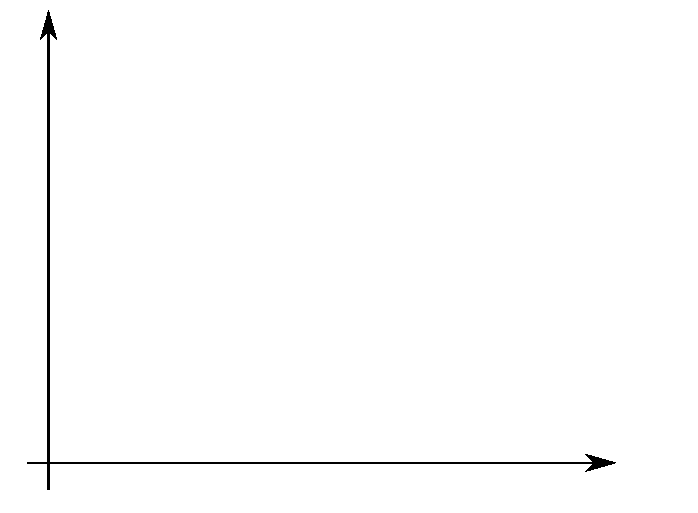
\includegraphics[width=0.85\textwidth]{figs/mobilerobot.png}
    \def\svgwidth{0.85\textwidth}
    \import{./figs/kinematics/}{mobilerobot.pdf_tex}
    \caption{Mobile robot with local coordinate system \{R\} and world frame \{I\}. The arrows indicate the positive direction of position and orientation vectors.}
    \label{fig:mobilerobot}
\end{figure}

Notice that the positioning of the coordinate frames and their orientation are arbitrary. Here, we choose to place the coordinate system in the center of the robot's axle and align $^Rx$ with its default driving direction.
In order to calculate the robot's position in the inertial frame, we need to first find out how speed in the robot coordinate frame maps to speed in the inertial frame.
This can be done again by employing trigonometry. There is only one complication: a movement into the robot's $x-$axis might lead to movement along both the $x-$axis and the $y-$axis of the world coordinate frame ${I}$. By looking at \cref{fig:mobilerobot}, we can derive the following components to $\dot{x}_I$. First,
\begin{equation}
\dot{x}_{I,x}=cos(\theta) \dot{x}_R.
\end{equation}

There is also a component of motion coming from $ \dot{y}_R$ (ignoring the kinematic constraints for now, see below).  For negative $ \theta$, as in \cref{fig:mobilerobot}, a move along $y_R$ would let the robot move into positive $ X_I$ direction. The projection from $ \dot{y}_R$ is therefore given by
\begin{equation}
\dot{x_{I,y}}=-sin(\theta)\dot{y_R}.
\end{equation}
We can now write
\begin{equation}
\dot{x_I}=cos(\theta) \dot{x_R} - sin(\theta) \dot{y_R}.
\end{equation}
Similar reasoning leads to:
\begin{equation}
\dot{y_I}=sin(\theta) \dot{x_R} + cos(\theta) \dot{y_R}
\end{equation}
and
\begin{equation}
\dot{\theta_I}=\dot{\theta_R}
\end{equation}
which is the case because both robot's and world coordinate system share the same z-axis in this example. We can now conveniently write
\begin{equation}
\dot{\xi_I}=^I_RT(\theta)\dot{\xi_R}
\end{equation}
with
\begin{equation}
^I_RT(\theta)=\left[\begin{array}{ccc}
cos(\theta) & -sin(\theta) & 0 \\
sin(\theta) & cos(\theta) & 0 \\
0 & 0 & 1\end{array}\right]
\end{equation}

We are now left with the problem of how to calculate the speed $ \dot{\xi_R}$ in robot coordinates. For this, we make use of the \textsl{kinematic constraints}\index{Kinematic constraints} of the robotic wheels.
For a standard wheel in an ideal case scenario, the kinematic constraints are that every rotation of the wheel leads to strictly forward or backward motion and does not allow side-way motion or sliding. We can therefore calculate the forward speed of a wheel $ \dot{x}$ using its rotational speed $ \dot{\phi}$ (assuming the encoder value/angle is expressed as $ \phi$) and radius $ r$ by
\begin{equation}
\dot{x}=\dot{\phi}r.
\end{equation}
This becomes apparent when considering that the circumference of a wheel with radius $r$ is $2\pi r$. The distance a wheel rolls when turned by the angle $ \phi$ (in radians) is therefore $ x=\phi r$, see also \cref{fig:wheelrotation}, right. Taking the derivative of this expression on both sides leads to the above expression.

\begin{figure}[htb!]
    \centering
    % 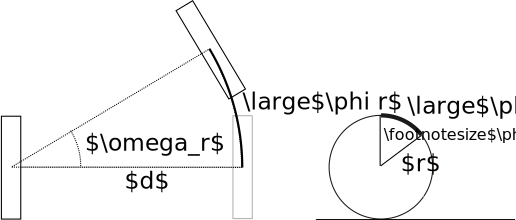
\includegraphics[width=0.9\textwidth]{figs/wheelrotation.png}
    \def\svgwidth{\textwidth}
    \import{./figs/kinematics/}{wheelrotation_2.pdf_tex}
    \caption{Left: Differential wheel robot pivoting around its left wheel first and its right wheel next. For infinitesimal motion, it is possible to decouple left and right wheel to simplify computation of the forward kinematics. Right: A wheel with radius $r$ moves by $\phi r$ when rotated by $\phi$ degrees.}
    \label{fig:wheelrotation}
\end{figure}

How each of the two wheels in our example contributes to the speed of the robot's center---where its coordinate system is anchored---requires the following trick: we calculate the contribution of each individual wheel while assuming all other wheels remaining un-actuated (see \cref{fig:wheelrotation}, left).
In this example, the left wheel will move of $r \phi_l$, and the right wheel will move of $r \phi_r$, which in the space of velocities will become $r\dot{\phi_l}$ and $r\dot{\phi_r}$ respectively.
Then, the distance traveled by the center point is exactly half of that traveled by each individual wheel, assuming the non-actuated wheel rotating around its ground contact point (\cref{fig:wheelrotation}). We can therefore write:
\begin{equation}
\dot{x_R}=\frac{1}{2}\left( r\dot{\phi_l} + r\dot{\phi_r} \right)=\frac{r\dot{\phi_l}}{2}+\frac{r\dot{\phi_r}}{2}
\end{equation}
given the speeds $ \dot{\phi_l}$ and $ \dot{\phi_r}$ of the left and the right wheel, respectively.

\begin{mdframed}
Think about how the robot's speed along its y-axis is affected by the wheel speed given the coordinate system in the drawing above. Think about the kinematic constraints that the standard wheels impose.
\end{mdframed}

Hard to believe at first, but the speed of the robot along its y-axis is always zero. This is because the constraints of the standard wheel tell us that the robot can never slide.
We are now left with calculating the rotation of the robot around its z-axis. This rotation can be seen when imaging the robot's wheels spinning in opposite directions. Then the robot does not move forward, but spins in place.
We will again consider each wheel independently. Assuming the left wheel to be non-actuated, spinning the right wheel forwards will lead to counter-clockwise rotation. Given an axle diameter (distance between the robot's wheels) $d$, we can now write
\begin{equation}
\omega_r d = \phi_r r
\end{equation}
with $\omega_r$ the angle of rotation around the left wheel (\cref{fig:wheelrotation}, left). Taking the derivative on both sides yields speeds and we can write
\begin{equation}
\dot{\omega_r} = \frac{\dot{\phi_r} r}{d}
\end{equation}
Adding the rotation speeds up (with the one around the right wheel being negative based on the right-hand grip rule), leads to:
%
\begin{equation}
\dot{\theta}=\frac{\dot{\phi_r} r}{d}-\frac{\dot{\phi_l} r}{d}
\end{equation}
%
Putting it all together, we can finally write:

\begin{equation}\label{eq:kinematics:forward:mobile}
\left[\begin{array}{c} \dot{x_I}\\\dot{y_I}\\\dot{\theta}\end{array}\right]=\left[\begin{array}{ccc}
cos(\theta) & -sin(\theta) & 0 \\
sin(\theta) & cos(\theta) & 0 \\
0 & 0 & 1\end{array}\right]\left[\begin{array}{c}\frac{r\dot{\phi_l}}{2}+\frac{r\dot{\phi_r}}{2}\\0\\\frac{\dot{\phi_r} r}{d}-\frac{\dot{\phi_l} r}{d}\end{array}\right]
\end{equation}

\subsubsection{From Forward Kinematics to Odometry}

\cref{eq:kinematics:forward:mobile} only provides us with the relationship between the robot's wheel speed and its speed in the inertial frame.
Calculating its actual pose in the inertial frame is known as \textsl{odometry}\index{Odometry}. Technically, it requires integrating \cref{eq:kinematics:forward:mobile} from 0 to the current time $T$.
As this is not possible but for very special cases, one can approximate the robot's pose by summing up speeds over discrete time intervals, or more precisely:
\begin{equation}
\left[\begin{array}{c} {x_I}(T)\\{y_I}(T)\\{\theta}(T)\end{array}\right]=
\int_0^T \left[\begin{array}{c} \dot{x_I}(t)\\\dot{y_I}(t)\\\dot{\theta}(t)\end{array}\right] dt \approx
\sum_{k=0}^{k=T}\left[\begin{array}{c} \Delta{x_I}(k)\\\Delta{y_I}(k)\\\Delta{\theta}(k)\end{array}\right]\Delta t
\end{equation} which can be calculated incrementally as
\begin{equation}\label{eq:odometry}
x_I(k+1)=x_I(k)+\Delta x (k) \Delta t
\end{equation}
using $\Delta x(k) \approx \dot{x_I}(t)$ and similar expressions for $y_I$ and $\theta$. Note that \cref{eq:odometry} is just an approximation. The larger $\Delta t$ becomes, the more inaccurate this approximation becomes as the robot's speed might change during the interval.

\begin{mdframed}
\noindent Don't let the notion of an integral worry you! As robots' computers are fundamentally discrete, integrals usually turn into sums, which are nothing than for-loops.
\end{mdframed}

\subsection{Forward kinematics of Car-like steering}\label{sec:kinematics:fwk:car}

Differential wheel drives are very popular in mobile robotics as they are very easy to build, maintain, and control.
Although not holonomic, a differential drive can approximate the function of a fully holonomic robot by first driving on the spot to achieve the desired heading and then driving straight.
Drawbacks of the differential drive are its reliance on a caster wheel, which performs poorly at high speeds, and difficulties in driving straight lines as this requires both motors to drive at the exact same speed.

These drawbacks are mitigated by car-like mechanisms, which are driven by a single motor and can steer their front wheels. This mechanism is known as ``Ackermann steering''. \index{Ackermann steering}
Ackermann steering should not be confused with ``turntable'' steering \index{Turntable steering} where the front wheels are fixed on an axis with central pivot point.
Instead, each wheel has its own pivot point and the system is constrained in such a way that all wheels of the car drive on circles with a common center point, avoiding skid.
As the Ackermann mechanism lets all wheels drive on circles with a common center point, its kinematics can be approximated by those of a tricycle with rear-wheel drive, or even simpler by a bicycle. This is shown in \cref{fig:ackermann}.

\begin{figure}[htb!]
    \centering
    % 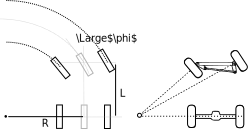
\includegraphics[width=0.9\textwidth]{figs/ackermann.png}
    \def\svgwidth{0.9\textwidth}
    \import{./figs/kinematics/}{ackermann.pdf_tex}
    \caption{Left: Kinematics of car-like steering and the equivalent bicycle model. Right: Mechanism of an Ackermann vehicle.}
    \label{fig:ackermann}
\end{figure}

Let the car have the shape of a box with length $L$ between rear and front axis. Let the center point of the common circle described by all wheels be distance $ R$ from the car's longitudinal center line. Then, the steering angle $ \phi$ is given by

\begin{equation}\label{eq:ackermann}
\tan \phi = \frac{L}{R}
\end{equation}

The angles of the left and the right wheel, $ \phi_l$ and $ \phi_r$ can be calculated using the fact that all wheels of the car rotate around circles with a common center point. With the distance between the two front wheels $l$, we can write:
\begin{eqnarray}
\frac{L}{R-l/2}&=\tan{(\phi_r)} \nonumber \\
\frac{L}{R+l/2}&=\tan{(\phi_l)}
\end{eqnarray}
This is important, as it allows us to calculate the resulting wheel angles resulting from a specific angle $\phi$ and test whether they are within the constraints of the actual vehicle.

Assuming the wheel speed to be $\dot{\omega}$ and the wheel radius $r$, we can calculate the speeds in the robot's coordinate frame as:
\begin{eqnarray}
\dot{x}_r&=&\dot{\omega}r \nonumber \\
\dot{y}_r&=&0\\
\dot{\theta}_r&=&\frac{\dot{\omega}r\tan\phi}{L} \nonumber
\end{eqnarray}
using (\ref{eq:ackermann}) to calculate the circle radius $R$.

\section{Inverse Differential Kinematics}\label{sec:kinematics:diff:inv}

%\subsection{Inverse Kinematics using Feedback Control}\label{sec:kinematics:inverse:feedbackcontrol}

%As we can easily calculate the resulting pose for every possible joint angle combination using the forward kinematic equations (\cref{sec:kinematics:fwd}), we can calculate the error between desired and actual pose.
%This error actually provides us with a \textsl{direction of motion} that the end-effector needs to move toward so as to minimize such error.
%As we only need to move tiny bits at a time and can then re-calculate the error, this is an attractive method to generate a trajectory that moves the arm to where we want it go and thereby solves the inverse kinematics problem. This approach is also known as \emph{gradient descent}\index{Gradient Descent}.
T%his is even more effective for non-holonomic mobile robots, where solving the inverse kinematic problem requires us to find a sequence of actuation commands.
%A more formal way of doing this is to employ \textsl{feedback control}\index{Feedback Control}.
%In a nutshell, feedback control uses the error between actual and desired position to calculate a trajectory that drives the robot a little closer to its desired pose. The process is then repeated until the error is marginally small.
%This approach can not only be used for mobile robots, but also for manipulator arms with kinematics that are too complicated to solve analytically.


% Fortunately, there are simple numerical techniques that work reasonably well in such situations.
% One of them is known as the \textsl{inverse Jacobian}\index{Inverse Jacobian} technique.

It would now be desirable to just invert $J$ in \cref{eq:kinematics:diff:fwd} in order to calculate the necessary joint speeds for every desired end-effector speeds---a problem known as \textsl{Inverse Differential Kinematics}\index{Inverse Differential Kinematics}. Unfortunately, as any matrix $J$ is only invertible if the number of degrees of freedom in joint space $n$ equals the number of degrees of freedom in task space $m$, so that $ J$ is quadratic and has full rank.
In the case above, the velocity wrench $[v \ \omega]^T$ is $6-$dimensional, and this means that $n$ should be equal to $6$: therefore, inversion of $J$ is only possible if the robot under consideration is equipped with exactly $6$ actuators/joints.
If this is not the case, we can use the pseudo-inverse computation:
\begin{equation}
J^+=\frac{J^T}{JJ^T}=J^T(JJ^T)^{-1}\label{eq:kinematics:diff:pseudoinverse}
\end{equation}
As you can see, $J^T$ cancels from the equation leaving $1/J$, while being applicable to non-quadratic matrices.
We can now write a simple feedback controller\index{Feedback control} that drives our error $e$ as the difference between desired and actual position to zero:
\begin{equation}
\Delta{q}=-J^+e
\end{equation}
That is, we move each joint a tiny bit into the direction that minimizes our error $e$.
It can be easily seen that the joint speeds are only zero if $e$ has become zero.

This solution might or might not be numerically stable, depending on the current joint values. If the inverse of $J$ is mathematically not feasible, we speak of a \textsl{singularity}\index{Singularity} of the mechanism. This happens for example when two joint axes line up, therefore effectively removing a degree of freedom from the mechanism, or at the boundary of the workspace. As it happens very often in robotics, the concept of singularity has both a strong mathematical justification (the joint configuration is such that the Jacobian is not full rank any more), and a direct physical consequence: singularity configurations are to be avoided as no solution for the inverse differential kinematics problem exist and the robot might become unsafe to operate.
In a singularity, the solution to $ J^+$ ``explodes'' and joint speeds go to infinity. In order to work around this, we can introduce damping to the controller.

In this case, we do not only minimize the error, but also the joint velocities. The minimization problem then becomes:
\begin{equation}
\|J\Delta q-e\|+\lambda^2\|\Delta q\|^2
\end{equation}
where $\lambda$ is some constant. One can show that the resulting controller that achieves this has the form:
\begin{equation}
\Delta q=(J^TJ+\lambda^2 I)^{-1}J^+e
\end{equation}

This is known as the \textsl{Damped Least-Squares} method.\index{Damped Least-Squares Method} Problems with this approach are local minima and singularities of the mechanism, which might render this solution infeasible.

\subsection{Inverse Kinematics of Mobile Robots}\label{sec:kinematics:ik:mobile}

There is no unique relationship between the amount of rotation of a robot's individual wheels and its position in space; however, for simple holonomic platforms such as a robot on a track, we will treat the inverse kinematics problem at first only for the velocities of the local robot coordinate frame.
%
Let's first establish how to calculate the necessary speed of the robot's center given a desired speed $ \dot{\xi_I}$ in world coordinates. We can transform the expression $ \dot{\xi_I}=T(\theta)\dot{\xi_R}$ by multiplying both sides with the inverse of $ T(\theta)$:

\begin{equation}\label{eq:mbik}
T^{-1}(\theta)\dot{\xi_I}=T^{-1}(\theta)T(\theta)\dot{\xi_R}
\end{equation}
which leads to $ \dot{\xi_R}=T^{-1}(\theta)\dot{\xi_I}$. Here

\begin{equation}
T^{-1}=\left[\begin{array}{ccc}cos \theta & sin \theta & 0 \\ -sin \theta & cos \theta & 0 \\ 0 & 0 & 1\end{array}\right]
\end{equation}
which can be computed by performing the matrix inversion or by deriving the trigonometric relationships from the drawing.  Similarly to \cref{sec:kinematics:inverse:arm}, we can now solve \cref{eq:kinematics:forward:mobile}
% \begin{equation}
% \left[\begin{array}{c} \dot{x_R}\\\dot{y_R}\\\dot{\theta}\end{array}\right]=\left[\begin{array}{c}\frac{r\dot{\phi_l}}{2}+\frac{r\dot{\phi_r}}{2}\\0\\\frac{\dot{\phi_r} r}{d}-\frac{\dot{\phi_l} r}{d}\end{array}\right]
% \end{equation}
for $ \phi_l$, $ \phi_r$:
\begin{eqnarray}
\dot{\phi}_l &= (2\dot{x}_R - \dot{\theta}d)/2r\\
\nonumber
\dot{\phi}_r &= (2\dot{x}_R + \dot{\theta}d)/2r
\end{eqnarray}
allowing us to calculate the robot's wheel speed as a function of a desired $\dot{x}_R$ and $\dot{\theta}$, which can be calculated using (\ref{eq:mbik}).

Note that this approach does not allow us to deal with $\dot{y}_R \neq 0$, which might result from a desired speed in the inertial frame. Non-zero values for translation in y-direction are simply ignored by the inverse kinematic solution, and driving toward a specific point either requires feedback control (Section~\ref{sec:kinematics:ik:invjac}) or path planning (Chapter~\ref{chap:pathplanning}).

\subsubsection{Inverse kinematics of an omnidirectional robot}
Omnidirectional robots using ``Swedish wheels'' \index{Swedish Wheel} or ``Meccano wheels'' \index{Meccano Wheel} are common in factories and educational settings. A drawing of a swedish wheel is shown in Table \ref{tab:wheels}. It consists of an actuated wheels with non-actuated rollers around its circumference that are attached in a 45 degree angle.

Like the caster wheel, the Swedish wheel has full three degrees of freedom in the plane, but can enable omnidirectional motion of a robotic platform without the need to rotate. A typical four-wheel configuration is shown in Figure \ref{fig:swedishwheel}. Notice the arrangment of the wheels, and in particular the orientation of the rollers, which is critical for the operation as shown.

When actuated by itself, the wheel will perform a sideways motion that is perpendicular to the main axis of its rollers. When used in pairs, opposite directions of motions cancel out, resulting for example into forward motion as shown in Figure \ref{fig:swedishwheel}, top, center, or sideways motion, bottom, right. 


 \begin{figure}[htb!]
    \centering
    % 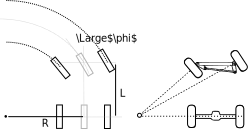
\includegraphics[width=0.9\textwidth]{figs/ackermann.png}
    \def\svgwidth{0.9\textwidth}
    \import{./figs/kinematics/}{swedishwheel.pdf_tex}
    \caption{Omni-directional robot using ``swedish wheels'' in different configurations. Each wheel has two velocity components, speed perpendicular to the wheel's main axis and speed of the rollers. Arrows on the robot body indicate the resulting direction of motion and rotation. }
    \label{fig:swedishwheel}
\end{figure}

Similar to a differential wheel platform, each wheel also exerts a rotation on the robot body. As the wheels are mounted off the center axle, each wheel contributes two moments. One around the horizontal axis with distance $h_i$ to the robot's center, the other around the vertical axis with distance $r_i$ to the robot's center (Figure \ref{fig:swedishwheel}, bottom, center). All combined, the rotation of each wheel will add up to the robot moving with velocities $v_x$, $v_y$ and $\omega_z$.

The velocity at each wheel has two components, the velocity of the $i$-th wheel perpendicular to its main axis $v_{i,m}$, and the velocity of the rollers $v_{i,r}$ that is either $+45\deg$ or $-45\deg$ to the wheel axis. Note that for the system to work, diagonally opposite wheels need to have the same angle. Let the angle of the roller of wheel $i$ be $\gamma_i$. We can now derive the following equations following \cite{maulana2015inverse}:
\begin{equation}\label{eq:swedish1}
v_{i,m}+v_{i,r}\cos(\gamma_i) = v_x - h_i*\omega_z
\end{equation}
That is, the velocity components perpendicular to the wheel axis are equivalent to the forward velocity of the robot plus the velocity component at the wheel resulting from the robot's angular velocity. (Positive angular velocity will result into backward motion per definition of the robot coordinate system.) Similarly, we can write 
\begin{equation}\label{eq:swedish2}
v_{i,r}\sin(\gamma_i) = v_y+r_i*\omega_z
\end{equation}
Note that there is no lateral component to the main wheel's motion, as lateral motion can only be achieved via the rollers. 

Dividing (\ref{eq:swedish2}) by (\ref{eq:swedish1}) and solving for $v_i$ results into
\begin{equation}
v_i=v_x-h_i\omega_z-\frac{v_y+r_i\omega_z}{\tan{\gamma_i}}
\end{equation}
With $h_i \in h =\{h,-h,h,-h\}$, $r_i \in r=\{r,r,-r,-r\}$ and 
$\gamma_i \in \gamma=\{-45\deg,+45\deg,+45\deg,-45\deg\}$ to reflect the different configuration of each wheel, we can derive an expression for the controllable wheel velocities $v_{i,m}$

\begin{eqnarray}
v_{1,m} &=& v_x+v_y+r\omega_z-h\omega_z \\
v_{2,m} &=& v_x-v_y-r\omega_z+h\omega_z \nonumber\\
v_{3,m} &=& v_x-v_y+r\omega_z-h\omega_z \nonumber\\
v_{4,m} &=& v_x+v_y-r\omega_z+h\omega_z \nonumber
\end{eqnarray}

With $v_{i,m}=R\omega_i$ and $R$ the radius of each Swedish wheel, we can now compute the required wheel velocity for any desired robot velocity $v_x$, $v_y$, and $\omega_z$. 

\subsubsection{Feedback control for mobile robots}\label{sec:fbmobile}

Assume the robot's position given by $x_r, y_r$ and $\theta_r$ and the desired pose as $x_g, y_g$ and $\theta_g$---with the subscript $g$ indicating ``goal''.
We can now calculate the error in the desired pose by:
\begin{eqnarray}
\rho  &=& \sqrt{(x_r-x_g)^2+(y_r-y_g)^2} \nonumber \\
\alpha&=& \tan^{-1}{\frac{y_g-y_r}{x_g-x_r}}-\theta_r \\
\eta  &=& \theta_g-\theta_r\ , \nonumber
\end{eqnarray}
which is illustrated in Figure~\ref{fig:trajectorygen}.
These errors can be converted directly into robot's speeds, for example using a simple proportional controller with gains $p_1$, $p_2$ and $p_3$:
\begin{eqnarray}
\dot{x} &=& p_1 \rho\\
\dot{\theta} &=& p_2 \alpha + p_3 \eta
\end{eqnarray}
which will let the robot drive in a curve until it reaches the desired pose.

\begin{figure}
    \centering
    % 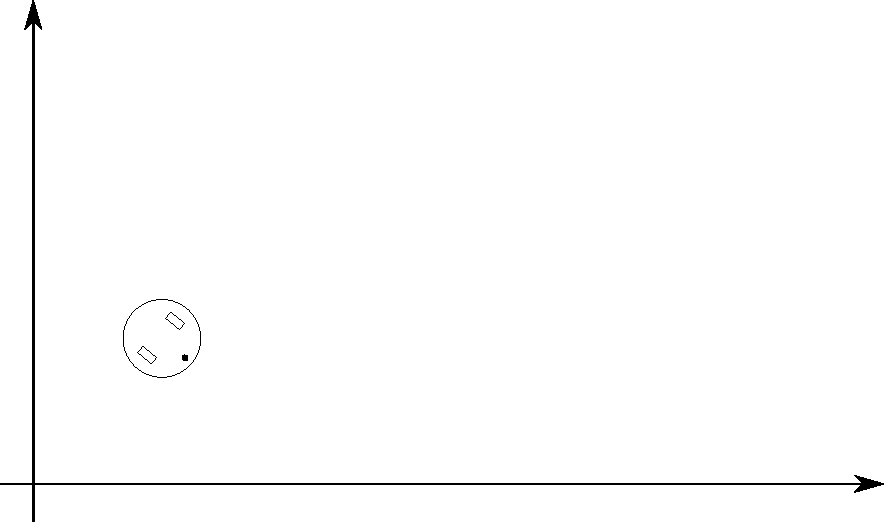
\includegraphics[width=\textwidth]{figs/trajectorygen.png}
    \def\svgwidth{\textwidth}
    \import{./figs/kinematics/}{trajectorygen.pdf_tex}
    \caption{Difference in desired and actual pose as a function of distance $\rho$, bearing $\alpha$ and heading $\eta$.}
    \label{fig:trajectorygen}
\end{figure}


\subsection{Under-actuation and Over-actuation}\label{sec:kinematics:diff:underover}

As detailed at the beginning of this Chapter, kinematics is concerned with analyzing the mapping between our control variables (i.e. the robot's motors represented by the $n$ DoFs in joint space) and their effect on the motion of the robot (our $m$ DoFs in task/configuration space). These two spaces might have different dimensionality, and the relation between these two dimensions greatly affects how we can solve the kinematic problem. It is convenient to analyze these differences by looking at the Jacobian $J$, since the size of the matrix is $m \times n$; in all, we have three different conditions:

\begin{itemize}
\item $n   =  m \rightarrow$ The robot is \textsl{fully actuated}. The Jacobian $J$ is square and full rank, and the forward kinematics equation is directly invertible;
\item $n \leq m \rightarrow$ The robot is \textsl{under actuated}, and the kinematics problem is \textsl{kinematically deficient}. The Jacobian $J$ is ``tall'', because there are more columns $m$ than rows $n$, and not invertible any more; the only way to solve the inverse kinematics problem is through the pseudo-inverse $J^+$ (and similar/more advanced approaches).
\item $n \geq m \rightarrow$ The robot is \textsl{over actuated}, and the kinematics problem is \textsl{kinematically redundant}. The Jacobian $J$ is ``fat'', because there are more rows $n$ than columns $m$, and not invertible any more; the only way to solve the inverse kinematics problem is through the pseudo-inverse $J^+$ (and similar/more advanced approaches). In this scenario, it is useful to determine the redundancy coefficient $n-m$ which affects the space of solutions of the inverse kinematic problem.
\end{itemize}

Over- and under-actuation are important design considerations to keep in mind when choosing a robot for a particular task.
In a \textsl{kinematically deficient} scenario, the robot is not capable of full motion in task space, as it does not have sufficient degrees of freedom in joint space to ``cover'' every possible configuration in task space. This does not mean that the robot is useless! It can still perform tasks---just not \textsl{every} possible task you might ask it to perform.
Conversely, if the problem is \textsl{kinematically redundant}, the robot has more joint DoFs available than it needs, and there exist an infinite number of inverse kinematics solutions in non-singular configurations.
Contrarily to what one may think, redundancy is actually a great feature to have in a robot system, in that it enables flexibility and versatility in solving the kinematic problem: that is, it is possible to choose \textsl{the best} solution among many, and one that satisfies additional constraints and requirements.
% As a matter of fact, the number of inverse kinematics solutions is $\infty^{n-m}$,
A human arm (without considering the hand) is a good example of a kinematically redundant manipulator, as it is equipped with $7$ DoFs in joint space ($3$ at the shoulder, $1$ at the elbow and $3$ at the wrist), whereas the task space is of dimension $6$ (i.e. the $3$ positions and $3$ orientations of the wrist).
This additional degree of mobility allows humans to reach for objects in multiple configurations, choose motions that are energy efficient, avoid obstacles, and more!
